\documentclass[border=10pt]{standalone}
\usepackage{tikz}
\usetikzlibrary{arrows.meta, shapes, calc}

\begin{document}

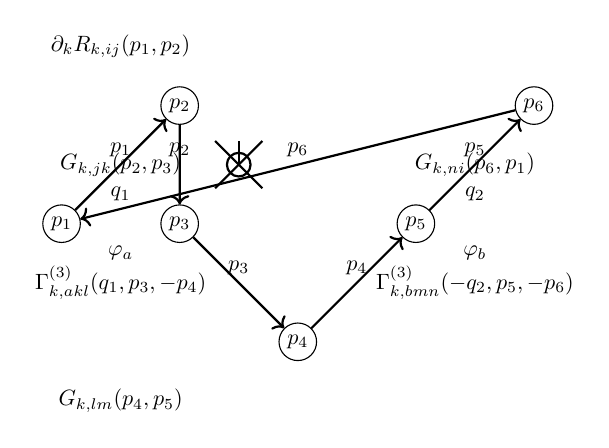
\begin{tikzpicture}[scale=1.5, every node/.style={scale=0.8}]
    % Nodes
    \node (p1) at (0,0) [circle, draw, fill=white, inner sep=2pt] {$p_1$};
    \node (p2) at (1,1) [circle, draw, fill=white, inner sep=2pt] {$p_2$};
    \node (p3) at (1,0) [circle, draw, fill=white, inner sep=2pt] {$p_3$};
    \node (p4) at (2,-1) [circle, draw, fill=white, inner sep=2pt] {$p_4$};
    \node (p5) at (3,0) [circle, draw, fill=white, inner sep=2pt] {$p_5$};
    \node (p6) at (4,1) [circle, draw, fill=white, inner sep=2pt] {$p_6$};
    
    % Arrows and labels
    \draw[->, thick] (p1) -- node[above] {$p_1$} (p2);
    \draw[->, thick] (p2) -- node[above] {$p_2$} (p3);
    \draw[->, thick] (p3) -- node[above] {$p_3$} (p4);
    \draw[->, thick] (p4) -- node[above] {$p_4$} (p5);
    \draw[->, thick] (p5) -- node[above] {$p_5$} (p6);
    \draw[->, thick] (p6) -- node[above] {$p_6$} (p1);
    
    % Mathematical notations
    \node at (0.5, 1.5) {$\partial_k R_{k,ij}(p_1, p_2)$};
    \node at (0.5, 0.5) {$G_{k,jk}(p_2, p_3)$};
    \node at (3.5, 0.5) {$G_{k,ni}(p_6, p_1)$};
    \node at (0.5, -0.5) {$\Gamma_{k,akl}^{(3)}(q_1, p_3, -p_4)$};
    \node at (3.5, -0.5) {$\Gamma_{k,bmn}^{(3)}(-q_2, p_5, -p_6)$};
    \node at (0.5, -1.5) {$G_{k,lm}(p_4, p_5)$};
    
    % Labels for arrows
    \node at (0.5, 0.25) {$q_1$};
    \node at (3.5, 0.25) {$q_2$};
    \node at (0.5, -0.25) {$\varphi_a$};
    \node at (3.5, -0.25) {$\varphi_b$};
    
    % Cross symbol
    \draw[thick] (1.5, 0.5) circle (0.1);
    \draw[thick] (1.5, 0.5) -- (1.5, 0.7);
    \draw[thick] (1.5, 0.5) -- (1.3, 0.3);
    \draw[thick] (1.5, 0.5) -- (1.7, 0.3);
    \draw[thick] (1.5, 0.5) -- (1.3, 0.7);
    \draw[thick] (1.5, 0.5) -- (1.7, 0.7);
    
\end{tikzpicture}

\end{document}